\documentclass[11pt]{article}

\usepackage{amsmath,amsthm,amssymb,amsfonts,mathrsfs,bbm,epsf,hyperref}
\usepackage[margin=1in]{geometry}
\usepackage{tikz} 
\usetikzlibrary{calc} 
\tikzset{>=latex}
\usetikzlibrary{matrix,positioning,fit,shapes.geometric}
\tikzset{
  mydot/.style={draw, circle, fill=black, inner sep=0pt, minimum size=4pt},
  myset/.style={draw, ellipse, very thick, inner sep=4pt},
}
\usetikzlibrary{arrows.meta}
\usepackage[usestackEOL]{stackengine}
\def\stackalignment{l}
\newcommand{\C}{\mathbb{C}}
\newcommand{\cj}{\overline}
\newcommand{\im}{\op{Im}}
\newcommand{\N}{\mathbb{N}}
\newcommand{\R}{\mathbb{R}}
\newcommand{\spa}{\operatorname{span}}
\newcommand{\tb}{\textbf}
\newcommand{\tn}{\textnormal}
\usepackage{algorithm}
\usepackage{algorithmic}
\usepackage{physics}
\usepackage[dvipsnames]{xcolor}
\usepackage{graphicx}
\usepackage{mathtools}
\usepackage{blkarray, bigstrut} %
\usepackage{amssymb}
\usepackage{tikz}
\usepackage{subcaption}
\usepackage{listings}
\usepackage[most]{tcolorbox}
\usepackage{adjustbox}
\usepackage{enumitem}
\usepackage{booktabs}
\usepackage{siunitx}
\usepackage{cancel}
\usepackage{wasysym}
\usepackage{caption}
\usepackage{tasks}

\tikzset{
box1/.style={draw=black, thick, rectangle,rounded corners, minimum height=4cm, minimum width=4cm},
box2/.style={draw=black, thick, rectangle, minimum height=4cm, minimum width=4cm},
}

\newcommand*{\vertbar}{\rule[-1ex]{0.5pt}{2.5ex}}
\newcommand*{\horzbar}{\rule[.5ex]{2.5ex}{0.5pt}}

\theoremstyle{definition}
\newtheorem*{prop}{Proposition}
\newtheorem*{cor}{Corollary}

\makeatletter
\renewcommand*\env@matrix[1][*\c@MaxMatrixCols c]{%
\hskip -\arraycolsep
\let\@ifnextchar\new@ifnextchar
\array{#1}}
\makeatother

\pagestyle{empty}

\begin{document}

\begin{center}
\noindent \large{\textbf{Probability Theory \hfill Fall 2025 \hfill}}
\end{center}

\section{Sequences and Series of Functions}
\label{sec:sequences-series}
\emph{Pointwise Convergence.} Suppose that $\{F_n\}$ is a sequence of functions on $D$ and the sequence of values $\{F_n(x)\}$ converges for each $x$ in some subset $S$ of $D$. Then we say that $\{F_n\}$ \emph{converges pointwise on $S$ to the limit function $F$}, defined by
\[
F(x) = \lim_{n\to\infty} F_n(x), \quad x \in S.
\]

\noindent
\emph{Uniform Convergence.} A sequence $\{F_n\}$ of functions defined on a set $S$ converges uniformly to the limit function $F$ on $S$ if
\[
    \lim_{n\to\infty} \|F_n - F\|_S = 0.
\]
Thus, $\{F_n\}$ converges uniformly to $F$ on $S$ if for each $\epsilon > 0$ there is an integer $N$ such that
\[
    \|F_n - F\|_S < \epsilon, \quad \text{if} \quad n \geq N.
\]

\begin{center}
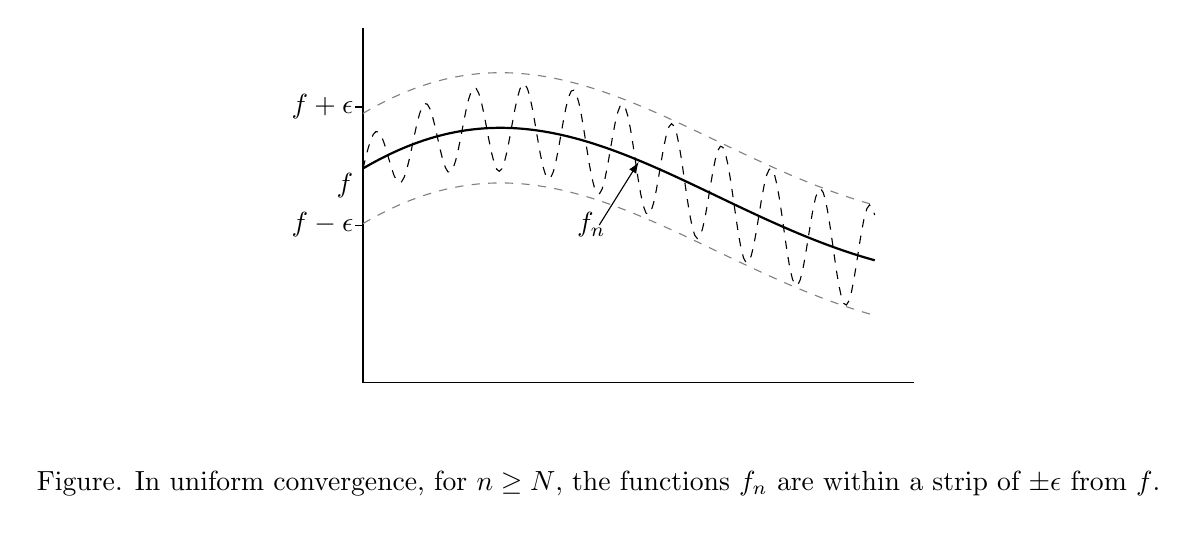
\begin{tikzpicture}
    % Axes
    \draw (0,0) -- (7,0); % x-axis
    \draw (0,0) -- (0,4.5); % y-axis

    % Labels for y-axis
    \node[left] at (0, 2.5) {$f$};
    \node[left] at (0, 3.5) {$f+\epsilon$};
    \node[left] at (0, 2) {$f-\epsilon$};

    % Dashed lines for f+epsilon and f-epsilon
    \draw[dashed, gray] plot[domain=0:6.5, samples=100] (\x, {2 + 1.5*exp(-0.1*\x) * sin(deg(\x/2 + 0.5)) + 0.7}); % f + epsilon
    \draw[dashed, gray] plot[domain=0:6.5, samples=100] (\x, {2 + 1.5*exp(-0.1*\x) * sin(deg(\x/2 + 0.5)) - 0.7}); % f - epsilon

    % The function f (the middle smooth line)
    \draw[thick] plot[domain=0:6.5, samples=100] (\x, {2 + 1.5*exp(-0.1*\x) * sin(deg(\x/2 + 0.5))});

    % The function fn (the wavy line)
    \draw [dashed] plot[domain=0:6.5, samples=200] (\x, {2 + 1.5*exp(-0.1*\x) * sin(deg(\x/2 + 0.5)) + 0.7*sin(deg(10*\x)) * (1 - 0.5*exp(-0.5*\x))});

    % Arrow and label for fn
    \draw[->] (3, 2) -- (3.5, 2.8);
    \node at (2.9, 2) {$f_n$};

    % Small tick marks on y-axis
    \draw (0, 2) -- (-0.1, 2);
    \draw (0, 3.5) -- (-0.1, 3.5);
    % \draw (0, 1.5) -- (-0.1, 1.5);
    \node[below=1cm] at (current bounding box.south) {Figure. In uniform convergence, for $n \ge N$, the functions $f_n$ are within a strip of $\pm \epsilon$ from $f$.};
\end{tikzpicture}
\end{center}

\noindent
\emph{Showing Pointwise and Uniform Convergence.}

\section{Measures}
\label{sec:measures}
\subsection{$\sigma$-algebra generated by a class.}
\label{subsec:measures:sigma-algebra-generated-class} If $\mathcal{A}$ is a class of subsets of $\Omega$, then the $\sigma$-algebra generated by $\mathcal{A}$, denoted by $\sigma(\mathcal{A})$, is defined as
\[
  \sigma \langle\mathcal{A}\rangle = \bigcap_{\mathcal{F} \in \mathcal{I}(\mathcal{A})} \mathcal{F},
\]
where $\mathcal{I}(\mathcal{A}) \equiv \{\mathcal{F} : \mathcal{A} \subset \mathcal{F} \text{ and } \mathcal{F} \text{ is a } \sigma\text{-algebra on } \Omega\}$ is the collection of all $\sigma$-algebras containing the class $\mathcal{A}$.
\\
$\sigma \langle\mathcal{A}\rangle$ can be considered as the smallest $\sigma$-algebra generated by $\mathcal{A}$. This definition doesn't give us any construction,. However, for each $\mathcal{A} \in \mathcal{P}(\Omega)$, we know that $\bigcap_{\mathcal{F} \in \mathcal{I}(\mathcal{A})} \mathcal{F} \subseteq \mathcal{P}(\Omega)$. Hence, there exists $\mathcal{P}(\Omega)$ which can serve as the $\sigma \langle\mathcal{A}\rangle$.
\\
\emph{Facts.}
\begin{enumerate}
    \item Suppose $\mathcal{G}$ is a $\sigma$-algebra, and $\mathcal{A} \subset \mathcal{G}$, then:
    \[\sigma \langle\mathcal{A}\rangle \subset \mathcal{G}\]
    \begin{proof}
       \[\sigma \langle\mathcal{A}\rangle = \bigcap_{\mathcal{F} \in \mathcal{I}(\mathcal{A})} \mathcal{F}\]
        Since $\mathcal{F}$s are $\sigma$-algebra, then one of them should be $\mathcal{G}$. Thus, its intersection with other $\sigma$-algebras is the subset of $\mathcal{G}$
        \[\bigcap_{\mathcal{F} \in \mathcal{I}(\mathcal{A})} \mathcal{F} \subset \mathcal{G}\]
        Hence
        \[\sigma \langle\mathcal{A}\rangle \subset \mathcal{G}\]
    \end{proof}
    \item Suppose $\mathcal{A}$, then:
    \[\sigma \langle\mathcal{A}\rangle = \mathcal{A}\]
    \begin{proof}
        Similar to (1).
    \end{proof}
    \item [] Corollary: 
    \[\sigma \langle \sigma\langle\mathcal{A}\rangle \rangle = \sigma \langle\mathcal{A}\rangle\]
    \item If $\mathcal{A} \subseteq \mathcal{B}$, then:
    \[\sigma \langle\mathcal{A}\rangle \subseteq \sigma \langle\mathcal{B}\rangle\]
\end{enumerate}

\subsection{$\sigma$-algebra generated by $\mathcal{C}$.}
\label{subsec:measures:sigma-algebra-generated-c}
Let $\Omega$ be an uncountable set (e.g., $\mathbb{R}$) and let $\mathcal{C}$ be the collection of all singleton sets, i.e.
\[
\mathcal{C}=\bigl\{\{\omega\}:\,\omega\in\Omega\bigr\}.
\]
Find the smallest $\sigma$-algebra generated by $\mathcal{C}$. Justify your answer.
\\
\emph{Answer.}
The following set with respect to $\Omega$ is $\sigma\langle \mathcal{C}\rangle$:
\[
\mathcal{F} = \{\,A \subset \Omega \mid A \text{ is countable or co-countable}\,\}.
\]
To show $\sigma\langle \mathcal{C}\rangle = \mathcal{F}$, we prove both inclusions: 
$\sigma\langle \mathcal{C}\rangle \subset \mathcal{F}$ and $\mathcal{F} \subset \sigma\langle \mathcal{C}\rangle$.

\begin{enumerate}
    \item $\sigma\langle \mathcal{C}\rangle \subset \mathcal{F}$.  
    Since each singleton set is countable, it follows that $\mathcal{C} \subset \mathcal{F}$. 
    Moreover, we have previously shown that $\mathcal{F}$ is a $\sigma$-algebra (In class, example 1.1.4). 
    Therefore, the smallest $\sigma$-algebra generated by $\mathcal{C}$, namely $\sigma\langle \mathcal{C}\rangle$, must be contained in $\mathcal{F}$. 

    \item $\mathcal{F} \subset \sigma\langle \mathcal{C}\rangle$.  
    Let $A \in \mathcal{F}$. Then either $A$ is countable or $A^c$ is countable, leaving two cases:
    \begin{enumerate}
        \item If $A$ is countable, we can write $A$ as a countable union of singletons: 
        \[
        A = \bigcup_{n \geq 1} \{a_n\}.
        \]
        Since $\sigma\langle \mathcal{C}\rangle$ contains $\mathcal{C}$ and is closed under countable unions, it follows that $A \in \sigma\langle \mathcal{C}\rangle$.
        
        \item If $A^c$ is countable, then by the same reasoning $A^c \in \sigma\langle \mathcal{C}\rangle$. 
        Since $\sigma\langle \mathcal{C}\rangle$ is closed under complementation, we conclude that $A = (A^c)^c \in \sigma\langle \mathcal{C}\rangle$. 
    \end{enumerate}
\end{enumerate}


\subsection{Topological Space.}
\label{subsec:measures:topological-space} A \emph{topological space} is a pair $(\mathbb{S}, \mathcal{T})$ where $\mathbb{S}$ is a nonempty set and $\mathcal{T}$ is a collection of subsets of S such that
\begin{enumerate}[label=(\roman*), itemsep=0.5em, topsep=0.5em]
  \item $\mathbb{S} \in \mathcal{T}$,
  \item $\mathcal{O}_1, \mathcal{O}_2 \in \mathcal{T} \Rightarrow \mathcal{O}_1 \cap \mathcal{O}_2 \in \mathcal{T}$, and
  \item $\{\mathcal{O}_\alpha : \alpha \in I\} \subset \mathcal{T} \Rightarrow \bigcup_{\alpha \in I} \mathcal{O}_\alpha \in \mathcal{T}$.
\end{enumerate}
\begin{enumerate}
    \item Smallest Topology (Indiscrete Topology)
    \begin{itemize}
        \item [] The topology is
          \[
             \mathcal{T}_{\min} = \{\varnothing, S\}.
          \]
        \item [] The topological space is
          \[
              (S, \{\varnothing, S\}).        
          \]
    \end{itemize}
    \item Largest Topology (Discrete Topology)
    \begin{itemize}
        \item [] The topology is
          \[
             \mathcal{T}_{\max} = \mathcal{P}(S),
          \]
          the power set of $S$.
        \item [] The topological space is
          \[
              (S, \mathcal{P}(S)).        
          \]
          every subset of $S$ is open.
    \end{itemize}
\end{enumerate}
\subsection{Metric Space.}
\label{subsec:measures:metric-space} A \emph{metric space} is a pair $(\mathbb{S},d)$ where $\mathbb{S}$ is a nonempty set and $d$ is a function from $\mathbb{S} \times \mathbb{S} \to \mathbb{R}^+$ satisfying 
\begin{enumerate}[label=(\roman*), itemsep=0.5em, topsep=0.5em]
    \item $d(x,y) = d(y,x)$ for all $x, y \in \mathbb{S}$,
    \item $d(x,y) = 0$ iff $x=y$, and
    \item $d(x,z) \le d(x,y) + d(y,z)$ for all $x,y,z$ in $\mathbb{S}$ (triangle inequality)
\end{enumerate}
The function $d$ is called a metric on $\mathbb{S}$. 
\\
Any Euclidean space $\mathbb{R}^n (1 \le n < \infty)$ is a metric space under any one of the following metrics:
\\
\begin{enumerate}[label=(\alph*), itemsep=1.5em, topsep=0.5em]
    \item For $1 \le p < \infty$, $d_p(x,y) = \left( \sum_{i=1}^n |x_i - y_i|^p \right)^{1/p}$.

    \item $d_\infty(x,y) = \max_{1 \le i \le n} |x_i - y_i|$.

    \item For $0 < p < 1$, $d_p(x,y) = \sum_{i=1}^n |x_i - y_i|^p$.
\end{enumerate}
A metric space $(\mathbb{S},d)$ is a topological space where a set $\mathcal{O}$ is open if for all $x \in \mathcal{O}$, there is an $\epsilon > 0$ such that $B(x,\epsilon) = \{y : d(y,x) < \epsilon\} \subset \mathcal{O}$.
\\
\subsection{Borel $\sigma$-algebras.}
\label{subsec:measures:borel-sigma-algebras} A particularly useful class of $\sigma$-algebras are those generated by open sets of a topological space. These are called Borel $\sigma$-algebras.
\\
\emph{example.}
Let $\mathcal{B}(\mathbb{R}^k)$ denote the Borel $\sigma$-algebra on $\mathbb{R}^k$, $1 \leq k < \infty$.  
Then,
\[
\mathcal{B}(\mathbb{R}^k) \equiv \sigma\langle \{ A : A \text{ is an open subset of } \mathbb{R}^k \} \rangle
\]
is also generated by each of the following classes of sets
\[
\begin{aligned}
\mathcal{O}_1 &= \{(a_1,b_1)\times \cdots \times (a_k,b_k) : -\infty \leq a_i < b_i \leq \infty, \, 1 \leq i \leq k \}; \\
\mathcal{O}_2 &= \{(-\infty, x_1)\times \cdots \times (-\infty, x_k) : x_1, \ldots, x_k \in \mathbb{R}\}; \\
\mathcal{O}_3 &= \{(a_1,b_1)\times \cdots \times (a_k,b_k) : a_i, b_i \in \mathcal{Q}, \, a_i < b_i, \, 1 \leq i \leq k \}; \\
\mathcal{O}_4 &= \{(-\infty, x_1)\times \cdots \times (-\infty, x_k) : x_1, \ldots, x_k \in \mathcal{Q}\},
\end{aligned}
\]
where $\mathcal{Q}$ denotes the set of all rational numbers.
\begin{proof}
    In general, to prove  $\sigma\langle \mathcal{A}\rangle =  \sigma\langle \mathcal{B}\rangle$, it's enough to show $\mathcal{A} \subseteq  \sigma\langle \mathcal{B}\rangle$ and $ \mathcal{B} \subseteq  \sigma\langle \mathcal{A}\rangle$
\end{proof}
\noindent
On $\Omega = \mathbb{R}$, we typically use Borel $\sigma$-algebra.
\\
In general, on any space $\mathcal{S}$, with a topology $\tau$, we can have a Borel $\sigma$-algebra.
\[
\mathcal{B}(\mathbb{R}) \equiv \sigma\langle \{\text{Open sets in standard topology}\} \rangle
\]
Also, we can show that on $\mathbb{R}^k$ $L_p, \forall p$ generates the same open sets (topology). So,
\[
\mathcal{B}(\mathbb{R}^k) \equiv \sigma\langle \{\text{Open sets in standard topology}\} \rangle
\]
\subsection{$\pi$-system.}
\label{subsec:measures:pi-system} A class $\mathcal{C}$ of subsets of $\Omega$ is a \emph{$\pi$-system} or a \emph{$\pi$-class} if
\[
A, B \in \mathcal{C} \;\;\Rightarrow\;\; A \cap B \in \mathcal{C}.
\]
\begin{figure}[htbp]
  \centering
  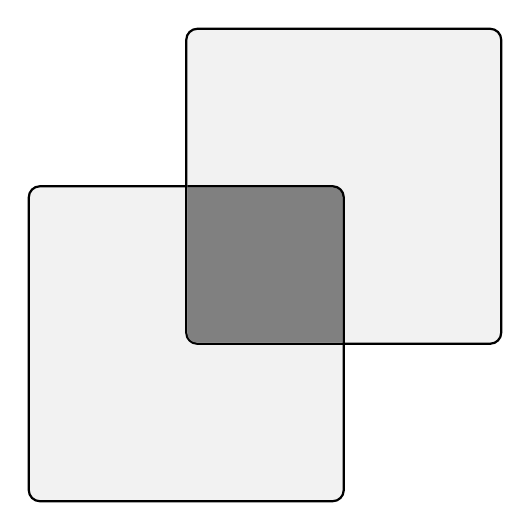
\begin{tikzpicture}
    \node[box1, fill=gray!10]  (c2) at (0,0) {};
    \node[box1, fill=gray!10] (c1) at (2,2) {};

    \fill[gray,thick]  (0+0.5*\pgflinewidth,2cm-0.5*\pgflinewidth)
      {[rounded corners=3pt+0.5\pgflinewidth] -- ++(2cm-\pgflinewidth,0)}
      -- ++(0,-2cm+\pgflinewidth)
      {[rounded corners=3pt+0.5\pgflinewidth] -- ++(-2cm+\pgflinewidth,0)}
      -- cycle;

    \draw[thick] (0+0.5*\pgflinewidth,2cm)
      {[rounded corners] -- ++(2cm-0.5\pgflinewidth,0)} -- ++(0,-2cm);
  \end{tikzpicture}

  \centering
    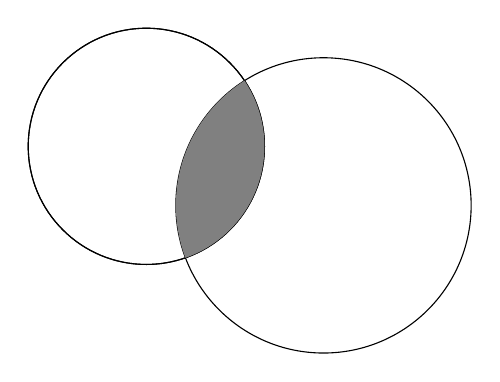
\begin{tikzpicture}[scale=0.75][thick]
       \draw (0,0) circle (2cm);
       \draw (3,-1) circle (2.5cm);
       \draw (0,0) node {};
       \draw (3.2,-1) node {};
       \draw [clip](0,0) circle (2cm);
       \fill[gray] (3,-1) circle (2.5cm);
    \end{tikzpicture}
  \caption{In $\mathbb{R}^2$, rectangles form a $\pi$-system because the intersection of two rectangles is a rectangle, but not circles.}
  \label{fig:rectangles-pi-system}
\end{figure}


\subsection{$\lambda$-class.}
\label{subsec:measures:lambda-class} A class $\mathcal{L}$ of subsets of $\Omega$ is a \emph{$\lambda$-system} or a \emph{$\lambda$-class} if
\begin{enumerate}
  \item[(i)] $\Omega \in \mathcal{L}$,
  \item[(ii)] $A,B \in \mathcal{L},\; A \subset B \;\Rightarrow\; B \setminus A \in \mathcal{L}$,
  \item[(iii)] $A_n \in \mathcal{L},\; A_n \subset A_{n+1}$ for all $n \geq 1 \;\Rightarrow\; \bigcup_{n \geq 1} A_n \in \mathcal{L}$.
\end{enumerate}
$\mathcal{F}$ a $\lambda$-class $\nRightarrow$ $\mathcal{F}$ is a $\sigma$-algebra.
\\
\emph{Example.} $\mathcal{F} = \{\Omega, \emptyset, \{a,b\}, \{c,d\}, \{a, c\}, \{b, d\} \}.$ $\mathcal{F}$ is a $\lambda$-class, but not a $\sigma$-algebra. 

\subsection{The $\pi$--$\lambda$ theorem.}
\label{subsec:measures:pi-lambda-theorem} If $\mathcal{C}$ is a $\pi$-system, then
\[
\lambda\langle \mathcal{C}\rangle \;=\; \sigma\langle \mathcal{C}\rangle .
\]
\begin{proof}
    The idea is to show $\lambda\langle \mathcal{C}\rangle \;\subseteq\; \sigma\langle \mathcal{C}\rangle$ and $\sigma\langle \mathcal{C}\rangle \;\subseteq\; \lambda\langle \mathcal{C}\rangle.$\\
    \begin{enumerate}
        \item $\lambda\langle \mathcal{C}\rangle \;\subseteq\; \sigma\langle \mathcal{C}\rangle$ \\
        Since every $\sigma$-algebra is a $\lambda$-system, $\sigma\langle \mathcal{C}\rangle$ is a $\lambda$-system containing $\mathcal{C}$.
        By minimality of $\lambda\langle \mathcal{C}\rangle$,
        \[
        \lambda\langle \mathcal{C}\rangle \subseteq \sigma\langle \mathcal{C}\rangle .
        \]

        \item $\sigma\langle \mathcal{C}\rangle \;\subseteq\; \lambda\langle \mathcal{C}\rangle$ \\
        Because $\lambda\langle \mathcal{C}\rangle$ is a $\lambda$-system, it satisfies:
        \begin{enumerate}
        \item [(i)] $\Omega \in \lambda\langle \mathcal{C}\rangle$,\\
        \item [(ii)] $A\in \lambda\langle \mathcal{C}\rangle \;\Rightarrow\; A^c=\Omega\setminus A \in \lambda\langle \mathcal{C}\rangle$,\\
        \item [(iii)] $A_1\subseteq A_2\subseteq \cdots,\ A_n\in \lambda\langle \mathcal{C}\rangle
        \ \Rightarrow\ \bigcup_{n\ge 1} A_n \in \lambda\langle \mathcal{C}\rangle$.
        \end{enumerate}

        We only need to verify finite unions are in $\lambda\langle \mathcal{C}\rangle$. That is, we need to prove: If $A \in \lambda\langle \mathcal{C}\rangle$ and $B \in \lambda\langle \mathcal{C}\rangle$, then
        \[
        A \cap B \in \lambda\langle \mathcal{C}\rangle.
        \]
        
        \bigskip
        
        First we'll prove: 
        
        If $A \in \lambda\langle \mathcal{C}\rangle$, $B \in \mathcal{C}$  
        \[
        \implies A \cap B \in \lambda\langle \mathcal{C}\rangle.
        \]
        
        \bigskip
        
        Also recall: 
        \[
        A \cup B = (A^c \cap B^c)^c.
        \]


        Define (good set argument):
        \[
        \lambda_1\langle \mathcal{C}\rangle = \{ A \in \lambda_1\langle \mathcal{C}\rangle : A \cap B \in \lambda_1\langle \mathcal{C}\rangle, \; \forall B \in \mathcal{C}\}.
        \]
        
        Clearly, $\mathcal{C} \subseteq \lambda_1\langle \mathcal{C}\rangle$.
        
        \medskip
        
        We will show $\lambda\langle \mathcal{C}\rangle = \lambda_1\langle \mathcal{C}\rangle$. Since $\lambda\langle \mathcal{C}\rangle$ is an $\lambda$-system, it suffices to prove $\lambda_1\langle \mathcal{C}\rangle$ is also an $\lambda$-system. Then, since $\lambda\langle \mathcal{C}\rangle$ is the smallest $\lambda$-system, $\lambda\langle \mathcal{C}\rangle \subseteq \lambda_1\langle \mathcal{C}\rangle$.
        
        \bigskip
        
        \textbf{Step:} Prove $\lambda_1\langle \mathcal{C}\rangle$ is a $\lambda$-system.
        
        \begin{enumerate}
            \item[(i)] $\Omega \in \lambda_1\langle \mathcal{C}\rangle$.
            \item[(ii)] If $A \in \lambda_1\langle \mathcal{C}\rangle$, then $A^c \in \lambda_1\langle \mathcal{C}\rangle$.
            \item[(iii)] If $A_i \in \lambda_1\langle \mathcal{C}\rangle$, pairwise disjoint, then $\bigcup_i A_i \in \lambda_1\langle \mathcal{C}\rangle$.
        \end{enumerate}
        
        \medskip
        
        Proof of (iii). Indeed, suppose $A_i \in \lambda_1\langle \mathcal{C}\rangle$.  
        We need to show
        \[
        \bigcup_i A_i \in \lambda_1\langle \mathcal{C}\rangle,
        \]
        i.e., for all $B \in \mathcal{C}$,
        \[
        \Big(\bigcup_i A_i\Big) \cap B \in \lambda\langle \mathcal{C}\rangle.
        \]
        
        But
        \[
        \Big(\bigcup_i A_i\Big) \cap B = \bigcup_i (A_i \cap B).
        \]
        
        Since $A_i \in \lambda_1\langle \mathcal{C}\rangle$, each $A_i \cap B \in \lambda\langle \mathcal{C}\rangle$. As $\lambda\langle \mathcal{C}\rangle$ is a $\lambda$-system, the union belongs to $\lambda\langle \mathcal{C}\rangle$.  
        
        \medskip
        
        Therefore,
        \[
        \bigcup_i A_i \in \lambda_1\langle \mathcal{C}\rangle, \qquad 
        \Big(\bigcup_i A_i\Big) \cap B \in \lambda\langle \mathcal{C}\rangle, \quad \forall B \in \mathcal{C}.
        \]


        (ii) Let $A,C \in \lambda\langle \mathcal{C}\rangle$. We will check that $(C \setminus A) \in \lambda\langle \mathcal{C}\rangle$.

        \medskip

        Since
        \[
        A \in \lambda\langle \mathcal{C}\rangle, \quad A \cap B \in \lambda\langle \mathcal{C}\rangle \quad \forall B \in \mathcal{C},
        \]
        and
        \[
        C \in \lambda\langle \mathcal{C}\rangle, \quad C \cap B \in \lambda\langle \mathcal{C}\rangle \quad \forall B \in \mathcal{C},
        \]
        we consider
        \[
        (C \setminus A) \cap B.
        \]
        
        \medskip
        
        Now,
        \[
        (C \setminus A) \cap B 
        = C \cap A^c \cap B
        = C \cap (A \cap B)^c.
        \]
        
        For some $B \in \mathcal{C}$ we have $A \cap B \in \lambda\langle \mathcal{C}\rangle$.  
        Thus $(A \cap B)^c \in \lambda\langle \mathcal{C}\rangle$.  
        Since also $C \in \lambda\langle \mathcal{C}\rangle$, it follows that
        \[
        (C \cap B) \cap (A \cap B)^c \in \lambda\langle \mathcal{C}\rangle.
        \]
        
        Hence $(C \setminus A) \cap B \in \lambda\langle \mathcal{C}\rangle$ for all $B \in \mathcal{C}$.  
        Therefore,
        \[
        C \setminus A \in \lambda\langle \mathcal{C}\rangle.
        \]
        
        \medskip
        
        This shows that $\lambda\langle \mathcal{C}\rangle$ is a $\lambda$-system. Therefore,
        \[
        \lambda_1\langle \mathcal{C}\rangle = \lambda\langle \mathcal{C}\rangle.
        \]
        
        That is, for all $A \in \lambda\langle \mathcal{C}\rangle$ and all $B \in \mathcal{C}$,
        \[
        A \cap B \in \lambda\langle \mathcal{C}\rangle.
        \]


        \noindent
        \textbf{(Same statement as above)}  
        \[
        \forall B \in \lambda\langle \mathcal{C}\rangle, \quad \forall A \in \mathcal{C} \;\;\implies\;\; A \cap B \in \lambda\langle \mathcal{C}\rangle.
        \]
        
        \bigskip
        
        \textbf{2.} Define
        \[
         \lambda_2\langle \mathcal{C}\rangle := \{ A \in \lambda\langle \mathcal{C}\rangle : A \cap B \in \lambda\langle \mathcal{C}\rangle, \;\; \forall B \in \mathcal{C}\}.
        \]
        
        We will prove:
        \[
         \lambda_2\langle \mathcal{C}\rangle = \lambda\langle \mathcal{C}\rangle \qquad \text{(end of proof).}
        \]
        
        \medskip
        
        \textit{Note:} $\mathcal{C} \subseteq  \lambda_2\langle \mathcal{C}\rangle$ (from the first step).  
        Indeed, if $A \in \mathcal{C}$, then from \((*)\), $A \in  \lambda_2\langle \mathcal{C}\rangle$.
        
        \medskip
        
        Now we will show that $ \lambda_2\langle \mathcal{C}\rangle$ is a $\lambda$-system.  
        Since $\mathcal{C} \subseteq  \lambda_2\langle \mathcal{C}\rangle$, this will imply
        \[
         \lambda_2\langle \mathcal{C}\rangle \supseteq \lambda\langle \mathcal{C}\rangle
        \]
        and hence
        \[
         \lambda_2\langle \mathcal{C}\rangle = \lambda\langle \mathcal{C}\rangle.
        \]
        
        \medskip
        
        Therefore, the proof is the same (or similar) to the first part of the argument. 
    \end{enumerate}
\end{proof}

    \emph{Corollary.}
    If $\mathcal{C}$ is a $\pi$-system and $\mathcal{L}$ is a $\lambda$-system containing $\mathcal{C}$, then $\mathcal{L} \supseteq \sigma(\mathcal{C})$.
    \begin{proof}
        $\sigma\langle\mathcal{C}\rangle = \lambda\langle \mathcal{C}\rangle \subset \mathcal{L}$
    \end{proof}


    \subsection{Measure}
    \label{subsec:measures:measure}
    Let $\Omega$ be a nonempty set and $\mathcal{F}$ be an algebra on $\Omega$.
    A set function $\mu$ on $\mathcal{F}$ is called a \emph{measure} if
    \begin{enumerate}[label=(\alph*)]
      \item [(i)] $\mu(A) \in [0,\infty]$ for all $A \in \mathcal{F}$;
      \item [(ii)] $\mu(\emptyset)=0$;
      \item [(iii)] for any disjoint collection of sets $A_1,A_2,\dots \in \mathcal{F}$ with $\bigcup_{n\ge 1} A_n \in \mathcal{F}$,
      \[
        \mu\!\left(\bigcup_{n\ge 1} A_n\right) \;=\; \sum_{n=1}^{\infty} \mu(A_n).
      \]
    \end{enumerate}
    
    \subsubsection{Proposition}
    \label{subsubsec:measures:measure:proposition-monotonicity}
    Let $(\Omega, \mathcal{F}, \mu)$ be a measure space. Then $\forall A, B \in \mathcal{F}$, such  that $A \subset B$:
    \begin{itemize}
        \item [(a)] $\mu(A) + \mu(B \backslash A) = \mu(B)$
        \item [(b)] $\mu(B \backslash A) = \mu(B) - \mu(A)$
        \item [(c)] $\mu(B) \geq \mu(A)$ (monotonicity)
    \end{itemize} 
    \begin{proof}
    \begin{itemize}
        \item [(a)] $B = A \cup (B \backslash A), \quad \text{($A$ and $B \backslash A$ are disjoint)} \implies \mu(B) = \mu(A) + \mu(B \backslash A)$
        \item [(b)] Based on $(a),$ 
        \begin{align*}
            & \mu(B) - \mu(A) = \mu(A) + \mu(B \backslash A) - \mu(A) \\
            \implies & \mu(B) - \mu(A) = \mu(B \backslash A)
        \end{align*}
        \item [(c)] Follows from $(a)$ and the fact that $\mu(A) \geq 0.$
    \end{itemize}
    \end{proof}
    
    \subsubsection{Proposition}
    \label{subsubsec:measures:measure:proposition-iff}
    Let $\Omega$ be a nonempty set and $\mathcal{F}$ be an algebra on $\Omega$ and $\mu$ be a set function on $\mathcal{F}$ with values in $[0, \infty]$ and with $\mu(\emptyset) = 0.$ Then, $\mu$ is a measure \emph{iff} $\mu$ satisfies:
    \begin{itemize}
        \item [$(iii)^i_{a}$] \textbf{Finite Additivity} $\forall A_1, A_2 \in \mathcal{F}$, with $A_1 \cap A_2 = \emptyset$,
        \[\mu(A_1 \cup A_2) = \mu(A_1) + \mu(A_2)\]
        \item [$(iii)^i_{b}$] \textbf{Monotone Continuity from Below of m.c.f.b in short} for any collection $\{A_n\}_{n \geq 1}$ of sets $\mathcal{F}$ such that $A_n \subset A_{n+1}$ for all $n \geq 1$ and $\bigcup_{n \geq 1} A_n \in \mathcal{F},$
        \[\mu \big (\cup_{n \geq 1} A_n \big ) = \lim_{n \to \infty} \mu (A_n)\]
    \end{itemize} 
    


    \subsubsection{Continuity from Above (mcfa).}
    \label{subsubsec:measures:measure:continuity-from-above}
    Suppose $(A_n)_{n \geq 1}$ is a decreasing sequence of measurable sets, i.e.
    \[
    A_1 \supseteq A_2 \supseteq A_3 \supseteq \cdots, 
    \qquad A = \bigcap_{n=1}^\infty A_n,
    \]
    and assume $\mu(A_1) < \infty$ (in particular, this holds if $\mu$ is a probability measure).  
    Then
    \[
    \mu(A) = \lim_{n \to \infty} \mu(A_n).
    \]
    
    \begin{proof}
    Define $B_n = A_n^c$. Then $(B_n)$ is an increasing sequence:
    \[
    B_1 \subseteq B_2 \subseteq \cdots,
    \qquad B = \bigcup_{n=1}^\infty B_n = \left(\bigcap_{n=1}^\infty A_n\right)^c.
    \]
    By continuity from below (mcfb),
    \[
    \mu(B) = \lim_{n \to \infty} \mu(B_n).
    \]
    Since $B_n = A_n^c$ and $B = A^c$, we have
    \[
    1 - \mu(A) = \lim_{n \to \infty} \big(1 - \mu(A_n)\big).
    \]
    Therefore,
    \[
    \mu(A) = \lim_{n \to \infty} \mu(A_n).
    \]
    \end{proof}
\newpage
\section{Integration}
\label{sec:integration}
Going forward, we will \emph{only} deal with $\sigma-$algebras.
\tikzset{set/.style={draw,circle,inner sep=0pt,align=center}}

\begin{figure}[htbp]
\centering
\setlength{\fboxrule}{.75pt}

% -------- Left box --------
\begin{minipage}[t]{0.45\linewidth}\centering
\fbox{\stackunder{$\mathcal{F}_1'$}{
  \fbox{\stackunder{%
    % Put a named TikZ node on F_1
    \tikz[remember picture,baseline=(Fone.base)] \node (Fone) {$\mathcal{F}_1$};%
  }{}}%
}}
\caption*{$(\Omega_1, \mathcal{F}_1, \mu_1)$, $\mathcal{F}_1 \subseteq \mathcal{F}_1'$}
\end{minipage}
\hfill
% -------- Right box --------
\begin{minipage}[t]{0.45\linewidth}\centering
\fbox{\stackunder{$\mathcal{F}_2$}{
  \fbox{\stackunder{%
    % Put a named TikZ node on F_2
    \tikz[remember picture,baseline=(Ftwo.base)] \node (Ftwo) {$\mathcal{F}_2'$};%
  }{}}%
}}
\caption*{$(\Omega_2, \mathcal{F}_2, \mu_2)$, $\mathcal{F}_2' \subseteq \mathcal{F}_2$}
\end{minipage}

% -------- Overlay arrows between the two labels --------
\begin{tikzpicture}[remember picture,overlay]
  % Solid arrow: F_1 -> F_2
  \draw[-{Latex[length=3mm]}] (Fone.east) to[bend left=18] node[midway, above, sloped] {$f: \Omega_1 \to \Omega_2$} (Ftwo.west);
  % Dashed arrow: F_2 -> F_1
  \draw[dashed,-{Latex[length=3mm]}] (Ftwo.west) to[bend left=18] node[midway, below, sloped] {$f^{-1}$} (Fone.east);
\end{tikzpicture}
\caption{The function $f$ is called $\langle \mathcal{F}_1, \mathcal{F}_2\rangle-$measurable if $\forall A \in \mathcal{F}_2, f^-1(A) \in \mathcal{F}_1$, where $f^-1(A) = \{\omega \in \Omega_1: f(\omega) \in A\}.$ Note: if $f$ is $\langle \mathcal{F}_1, \mathcal{F}_2\rangle-$measurable then is $\langle \mathcal{F}_1', \mathcal{F}_2'\rangle-$measurable.}
\end{figure}
\noindent
Note: If the left side (domain) has a probability measure, call it $P$, and the right hand side (range) has $(\Omega_2, \mathcal{F}_2) = (\mathbb{R}, \mathcal{B}(\mathbb{R}))$, then a measurable transformation is a random variable, and is denoted as $X, Y,$etc. (instead of $f$, $g$, etc.)
\\
\begin{center}
    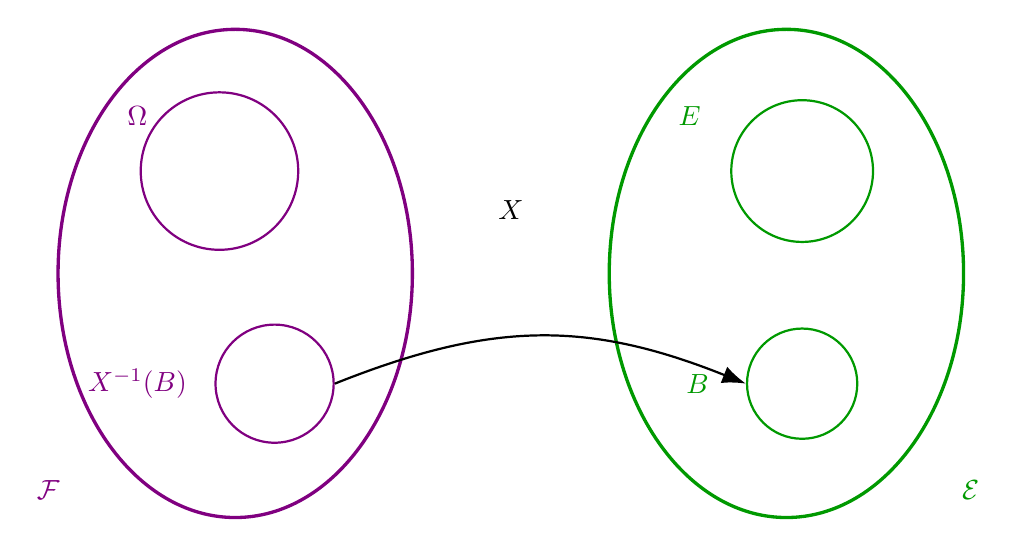
\begin{tikzpicture}[>=Latex, thick]
  % styles
  \tikzset{
    leftset/.style  ={draw, very thick, color=violet},
    rightset/.style ={draw, very thick, color=green!60!black},
    lcircle/.style  ={draw, color=violet, thick},
    rcircle/.style  ={draw, color=green!60!black, thick}
  }

  % Left sigma-algebra (F)
  \node[leftset, ellipse, minimum width=4.5cm, minimum height=6.2cm] (F) at (0,0) {};
  % little circles inside left
  \node[lcircle, circle, minimum size=2cm] (OmegaBlob) at (-0.2,1.3) {};
  \node[lcircle, circle, minimum size=1.5cm] (XinvB) at (0.5,-1.4) {};
  % labels on left
  \node[anchor=west, color=violet] at (-1.5, 2.0) {$\Omega$};
  \node[anchor=west, color=violet] at (-2.0,-1.4) {$X^{-1}(B)$};
  \node[anchor=south east, color=violet] at (-2.1,-3) {$\mathcal{F}$};

  % Right sigma-algebra (E)
  \node[rightset, ellipse, minimum width=4.5cm, minimum height=6.2cm] (Eset) at (7,0) {};
  % little circles inside right
  \node[rcircle, circle, minimum size=1.8cm] (EBlob) at (7.2,1.3) {};
  \node[rcircle, circle, minimum size=1.4cm] (B) at (7.2,-1.4) {};
  % labels on right
  \node[anchor=west, color=green!60!black] at (5.5, 2.0) {$E$};
  \node[anchor=west, color=green!60!black] at (5.6,-1.4) {$B$};
  \node[anchor=south west, color=green!60!black] at (9.1,-3) {$\mathcal{E}$};

  % Arrow X : (Omega,F) -> (Ecal, E)
  \draw[-{Latex[length=3mm]}] (XinvB.east) .. controls +(2,0.8) and +(-2,0.8) .. (B.west);
  \node at (3.5,0.8) {$X$};
\end{tikzpicture}
\end{center}


\emph{\textbf{Example 1.}}
Let $(\Omega_1,\mathcal{F}_1)$ and $(\Omega_2,\mathcal{F}_2)$ be measurable spaces, and fix a point $c\in\Omega_2$.
Define the constant map $f:\Omega_1\to\Omega_2$ by
\[
f(\omega)=c,\qquad \forall\,\omega\in\Omega_1 .
\]
Then $f$ is $\langle \mathcal{F}_1, \mathcal{F}_2\rangle-$measurable.

\begin{proof}
Take any $A\in\mathcal{F}_2$. Then
\[
f^{-1}(A)=\{\omega\in\Omega_1:\ f(\omega)\in A\}
=
\begin{cases}
\varnothing, & c\notin A,\\[3pt]
\Omega_1, & c\in A.
\end{cases}
\]
Since $\varnothing,\Omega_1\in\mathcal{F}_1$, we have $f^{-1}(A)\in\mathcal{F}_1$ for every $A\in\mathcal{F}_2$; hence $f$ is measurable.
\end{proof}

% (Optional specialization)
% In particular, if $\Omega_2=\mathbb{R}$ and $\mathcal{F}_2=\mathcal{B}(\mathbb{R})$,
% every constant real-valued function on $(\Omega_1,\mathcal{F}_1)$ is measurable.
\noindent
\emph{\textbf{Example 2.}}
Let $(\Omega,\mathcal{F})$ be a measurable space, and consider
\[
f:(\Omega,\mathcal{F}) \to (\mathbb{R},\mathcal{B}(\mathbb{R})), 
\qquad f = \mathbf{1}_B,
\]
where $B \subseteq \Omega$ with $B \in \mathcal{F}$.

For any $A \in \mathcal{B}(\mathbb{R})$, we have
\[
f^{-1}(A) = \{\,\omega \in \Omega : f(\omega) \in A\,\}
=
\begin{cases}
\varnothing, & \{0,1\} \cap A = \varnothing, \\[4pt]
B^c, & 0 \in A,\, 1 \notin A, \\[4pt]
B,   & 0 \notin A,\, 1 \in A, \\[4pt]
\Omega, & 0,1 \in A.
\end{cases}
\]

Thus $f^{-1}(A)\in\mathcal{F}$ for all $A\in\mathcal{B}(\mathbb{R})$
if and only if $B \in \mathcal{F}$ (equivalently $B^c \in \mathcal{F}$).
Hence $\mathbf{1}_B$ is measurable if and only if $B \in \mathcal{F}$.

\noindent
\emph{\textbf{Example 3.}}
Measurable transformations induce partitions of $\Omega$;
the $\sigma$-algebra $\mathcal{F}_1$ must be a refinement of such a partition.

Let
\[
\Omega = \{a,b,c,d\}, \qquad 
\mathcal{F} \equiv \mathcal{F}_2 = \{\Omega, \varnothing, \{a\}, \{b,c,d\}\}.
\]

Define $f:\Omega \to \mathbb{R}$ by
\[
f(a)=1, \qquad f(b)=13, \qquad f(c)=13, \qquad f(d)=13.
\]

We check measurability:
for $A \in \mathcal{B}(\mathbb{R})$,
\[
f^{-1}(A) =
\begin{cases}
\varnothing, & \{1,13\}\cap A = \varnothing, \\[4pt]
\{a\}, & 1 \in A,\, 13 \notin A, \\[4pt]
\{b,c,d\}, & 1 \notin A,\, 13 \in A, \\[4pt]
\Omega, & 1,13 \in A.
\end{cases}
\]

Thus $f^{-1}(A)\in\mathcal{F}$ for all $A \in \mathcal{B}(\mathbb{R})$,
so $f$ is $\langle \Omega, \mathcal{F}_2\rangle-$measurable.
\\
However, consider $g:\Omega \to \mathbb{R}$ by
\[
g(a)=1, \qquad g(b)=2, \qquad g(c)=13, \qquad g(d)=-10.
\]
Then $g$ is not a $\langle \Omega, \mathcal{F}_2\rangle-$measurable, since $g^{-1}(\{13\}) = \{c\} \notin \mathcal{F}_2.$
\\
\emph{\textbf{Example 4.}}
Let 
\[
\Omega = \{H,T\}, \qquad 
\mathcal{F} = \mathcal{P}(\Omega) = \{\varnothing,\Omega,\{H\},\{T\}\}.
\]
Define a probability measure $P$ on $(\Omega,\mathcal{F})$ by
\[
P(\{H\}) = p, \qquad P(\{T\}) = q, \qquad 0 \leq p,q \leq 1, \quad p+q=1.
\]

Define a map $X:\Omega \to \mathbb{R}$ by
\[
X(H)=1, \qquad X(T)=0.
\]
That is, $X = \mathbf{1}_{\{H\}}$. Since $\{H\}\in\mathcal{F}$, $X$ is a valid random variable.

\medskip

For probabilities of events involving $X$, we compute:
\[
P(X=1) = P\big(\{\omega : X(\omega)=1\}\big) 
= P\big(X^{-1}(\{1\})\big)
= P(\{H\}) = p.
\]
Similarly,
\[
P(X=0) = q.
\]

\medskip

In general, for $A \in \mathcal{B}(\mathbb{R})$,
\[
P(X \in A) \;=\; P\big(X^{-1}(A)\big).
\]
This defines a new measure on $(\mathbb{R},\mathcal{B}(\mathbb{R}))$,
\[
P_X(A) := P\big(X^{-1}(A)\big),
\]
called the \emph{induced measure} (or, in statistics, the \emph{distribution of $X$}).
\end{document}


